\setchapterpreamble[u]{\margintoc}
\chapter{Integration in a Proof Assistant}
\labch{plugin}

\epigraph{God does not care about our mathematical difficulties. He integrates
empirically.}{\textbf{Albert Einstein}}

In the previous chapters, we introduced the \kl{Proof-by-Action} paradigm
(\refch{pba}), and tried to convince the reader that it is both theoretically
sound with its firm grounding in \kl{deep inference} \kl{proof theory}
(\refch{sfl} and \refch{sfl-classical}), and practically useful by analyzing
proofs of mathematical problems expressed within it (\refch{advanced}). We also
mentioned multiple times our prototype of interface implementing \kl{PbA} called
\kl{Actema}, and in particular the fact that it exists as a \emph{standalone}
web application with its own proof engine \cite{Actema:link}. This is
convenient for distributing it online as a publicly available website, so that
people can immediately try it out without the hassles of installation
procedures. However due to both historical choices in its design and lack of
human resources for development, \kl{Actema}'s proof engine is quite limited in
its features:
\begin{itemize}
  \itemAP it can only handle \kl{goals} expressed in many-sorted
    \intro{intuitionistic first-order logic} (\intro{iFOL}), whereas all
    state-of-the-art \kl{PAs} support \emph{\kl{higher-order}} logic in one form
    or another; and \kl{higher-order} features are crucial for formalizing many
    mathematical notions in a concise way, as witnessed by the example of
    \refsec{funcs};
  \item it does not implement a \emph{certified \kl(PA){kernel}} for checking
    proof objects, which makes it hard to trust and interoperate with;
  \item it has no mechanism for adding new \emph{mathematical notations}, only
    ad hoc support for arithmetical expressions. Thus formulas become very
    quickly impossible to read and manipulate;
  \item it has poor support for managing \emph{libraries} of definitions, lemmas
    and proofs, partly because of the previous items.
\end{itemize}
% Typically, the example studied in \refsec{funcs} cannot be carried out in the
% standalone version of Actema, because it lacks support for defining new
% predicates --- especially when they are higher-order like $\injective(\cdot)$
% --- as well as new notations for them like $\subseteq$ for set inclusion.

To address these limitations, and thus enable a confrontation of the \kl{PbA}
paradigm to real mathematical developments, we decided to build \kl{coq-actema},
a \kl{Coq} plugin that directly connects \kl{Actema} to a running instance of
the \kl{Coq} \kl{proof assistant} \cite{coq-actema}. The idea is that
\kl{Actema} should act as an enhanced graphical, interactive \kl{proof view}
that integrates in the usual text-based workflow of \kl{proof scripts}. Thus
instead of trying to turn \kl{Actema} into a full-fledged \kl{PA}, we exploit
the over 30 years of effort that have been put in the development of \kl{Coq},
and limit the role of \kl{Actema} to that of a novel frontend for building
proofs in \kl{Coq}. This shall open the way to more advanced experimentations
through the huge body of theories already developed in \kl{Coq}, and make the
\kl{PbA} paradigm visible to the large community of existing users of this
popular \kl{PA}.

\begin{remark}
  The same approach should be applicable in principle to any \kl{ITP} that
  supports at least \kl{iFOL}, and provides an interaction protocol for building
  proofs in a \kl{goal}-directed manner. This includes other popular \kl{PAs}
  such as \kl{Lean} and \kl{Isabelle}, but also more specialized software like
  the \intro{Why3} platform for deductive program verification
  \cite{boogie11why3}, the \intro{Meta-F*} framework in the proof-oriented
  programming language \intro{F*} \cite{martínez2019metaf}, or the
  \intro{EasyCrypt} toolset for the verification of cryptographic protocols
  \cite{Barthe2014}.
\end{remark}

The chapter is organized as follows: we start in \refsec{actema} by explaining
the architecture of the \kl{Actema} web application, which follows the standard
conceptual separation between frontend and backend. In \refsec{whyplugin}, we
reflect on some considerations that led us to the specific choice of a \kl{Coq}
plugin, in order to integrate \kl{Actema} with \kl{Coq}. Then in
\refsec{architecture} we present the architecture of the \kl{coq-actema} system,
which structures all interactions between the user, \kl{Coq} and \kl{Actema}.
\refsec{protocol} describes in more details the main usage scenario of
\kl{coq-actema}, following the flow of data and control between the different
processes involved. \refsec{compilation} explains how the various graphical
\kl{actions} performed by the user in \kl{Actema} are compiled into \kl{Coq}
\kl{tactics}, ultimately producing certified \kl{proof terms}. Finally in
\refsec{pluginfuture}, we discuss possible avenues for extending the usability
of \kl{coq-actema} to a broader class of \kl{Coq} \kl{goals}, as well as
prospective solutions to the problem of \kl{proof evolution} in our graphical
paradigm.

\section{Actema}\labsec{actema}

\AP At its core, \kl{Actema} is a web application made of two components: a
\emph{frontend} that implements the graphical interface with which the user
interacts, written in \kl{HTML}/\intro{CSS}/\kl{JavaScript} with the
\intro{Vue.js} framework \cite{Vuejs}; and a \emph{backend} that implements the
proof engine, written in \intro{OCaml} and compiled to \kl{JavaScript} (\kl{JS})
with \intro{js\_of\_ocaml} \sidecite{vouillon_bytecode_2014}. The two components
interact through an object-oriented API written in \kl{OCaml}, which is loaded
at runtime in the form of a \kl{JS} object called \texttt{engine}, and whose
methods can be called from the \kl[Vue.js]{Vue} components in the frontend.

The \texttt{engine} object provides various high-level methods for handling the
current \emph{\kl{proof state}}. Common operations include getting the list of open
\kl{subgoals}, querying available proof \kl{actions} on a \kl{subgoal}, or applying a given
proof \kl{action}. Lower-level methods are also available in other objects to inspect
the data of the \kl{proof state}. For instance,
$$\mathtt{engine.subgoals[0].context[0]}$$ will return an object representing
the first hypothesis of the first \kl{subgoal}; and this object itself exposes
an \texttt{html} method, which returns a string holding the \kl{HTML} code used to
display the statement of the hypothesis.

In the standalone version of \kl{Actema}, the proof engine takes care of
computing the new \kl{subgoals} stemming from \kl{actions} performed by the user. It
is thus responsible for defining the \emph{semantics} of proof \kl{actions}. It is
also in charge of various other tasks that process the logical data of the
\kl{proof state}, typically checking the \kl(sfl){validity} of \kl{linkages}
during a \kl{DnD} \kl{action}, which requires the use of a \kl{unification} algorithm
(see \refsec{validity}).

\section{Why a plugin?}\labsec{whyplugin}

\AP
Usually, \intro{integrated development environments} (\intro{IDEs}) for
\kl{Coq} live in an independent process, and exchange data with \kl{Coq} through
a high-level communication protocol: either the command line interface provided
by \texttt{coqtop}, \kl{Coq}'s default \intro{XML} protocol, or its improved
superset \intro{SerAPI} \sidecite{gallegoarias:hal_01384408}. In particular,
\kl{SerAPI} emerged from the development of \intro{jsCoq}
\sidecite{Gallego_Arias_2017}, an \kl{IDE} that runs entirely in web browsers by
embedding a version of \kl{Coq} compiled with \kl{js\_of\_ocaml}. Since
\kl{Actema} is also web-based and uses \kl{js\_of\_ocaml}, our first idea was
essentially to fork \kl{jsCoq} and replace its interface by that of \kl{Actema}.
However as noted by E. J. G. Arias, the \kl{SerAPI} protocol --- and in fact all
the other protocols turn out to be too high-level for our purpose. Typically we
need to (partially) translate \kl{Coq} \kl{goal}s into \kl{iFOL} \kl{goals},
which can be done much more easily with a direct access to \kl{Coq}'s low-level
API for manipulating \kl(PA){kernel} \kl{terms}.
% We also heavily rely on unification to interactively suggest valid
% actions on subterms of the goal, and none of the protocols implement unification
% queries.

Now, remember that \kl{Actema} is not meant as a full-fledged \kl{IDE} that can
manage the edition and execution states of the \kl{proof script}, but only as an
enhanced \kl{proof view} for manipulating already-parsed \kl{goals}. One should
think of \kl{Actema}'s \kl{actions} simply as a graphical frontend for invoking a new
set of \kl{tactics}. And this is precisely what the plugin system of \kl{Coq}
has been designed for: extending \kl{Coq} with new \kl{tactics}. Thus the
solution of a \kl{Coq} plugin made a lot more sense, with the important benefit
of ensuring compatibility with all existing \kl{IDEs}. This would also entail
easier adoption of \kl{Actema} into existing \kl{Coq} developments and
workflows.

In this setting, it is now the \kl{Coq} plugin which implements the semantics of
proof \kl{actions} as new \kl{tactics}, instead of \kl{Actema}'s backend. This allows
us to leverage the facilities already provided by \kl{Coq} to handle the
\kl{proof state} and generate \kl{proof terms} in the \kl{calculus of inductive
constructions}. This does not make the backend of \kl{Actema} completely
irrelevant however: we still need it so that \kl{Actema} can maintain its own,
\kl{first-order} version of the \kl{proof state}, with additional metadata used
to display and interact graphically with objects and statements. Also tasks
related to the querying of both display data and proof \kl{actions}, like the
\texttt{html} method and \kl{unification} algorithm mentioned in the previous
section, are at the time of writing of this thesis still performed in
\kl{Actema}'s backend. It is unclear to what extent this should rather be a
responsibility of the \kl{Coq} plugin, relegating \kl{Actema} to a pure role of
frontend to the \kl{PA}\sidenote{For instance in the \kl{ProofWidgets} framework
\cite{ayers_graphical_2021}, all these tasks are implemented in the
meta-programming language of \kl{Lean} (which is \kl{Lean} itself), making it
more extensible by (expert) users of the \kl{PA}.}.

\section{The coq-actema system}\labsec{architecture}

\begin{figure*}
  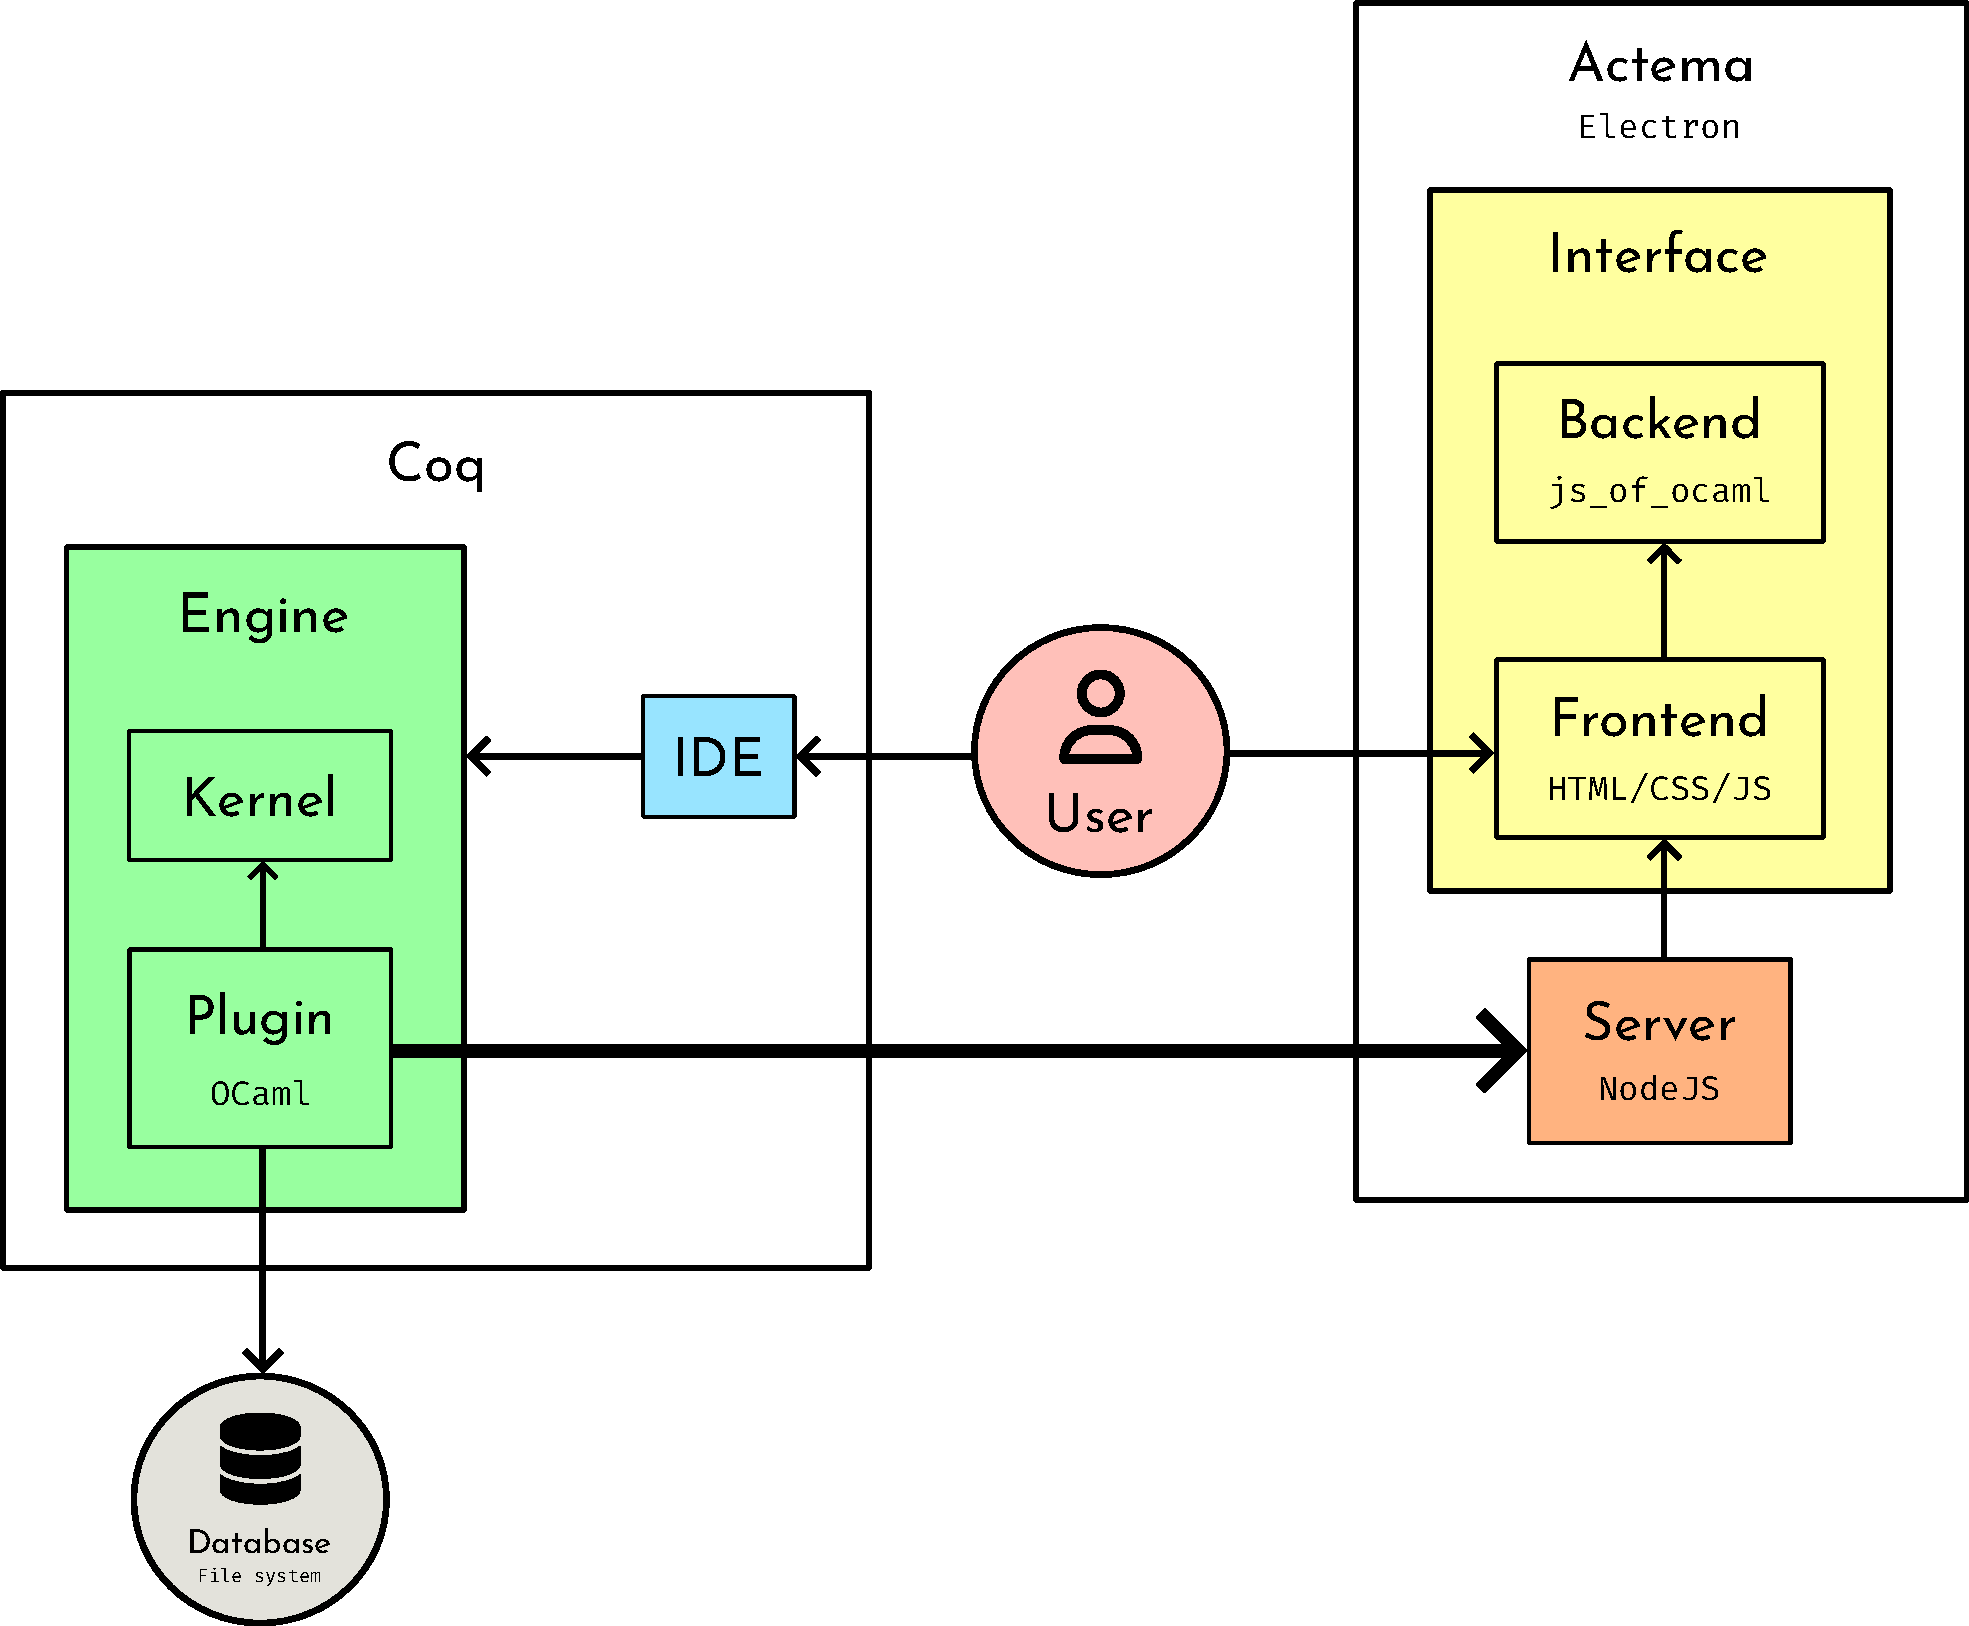
\includegraphics[width=1.3\textwidth]{archi.pdf}
  \caption{Architecture of the \kl{coq-actema} system}
  \labfig{archi}
\end{figure*}

\begin{figure*}
  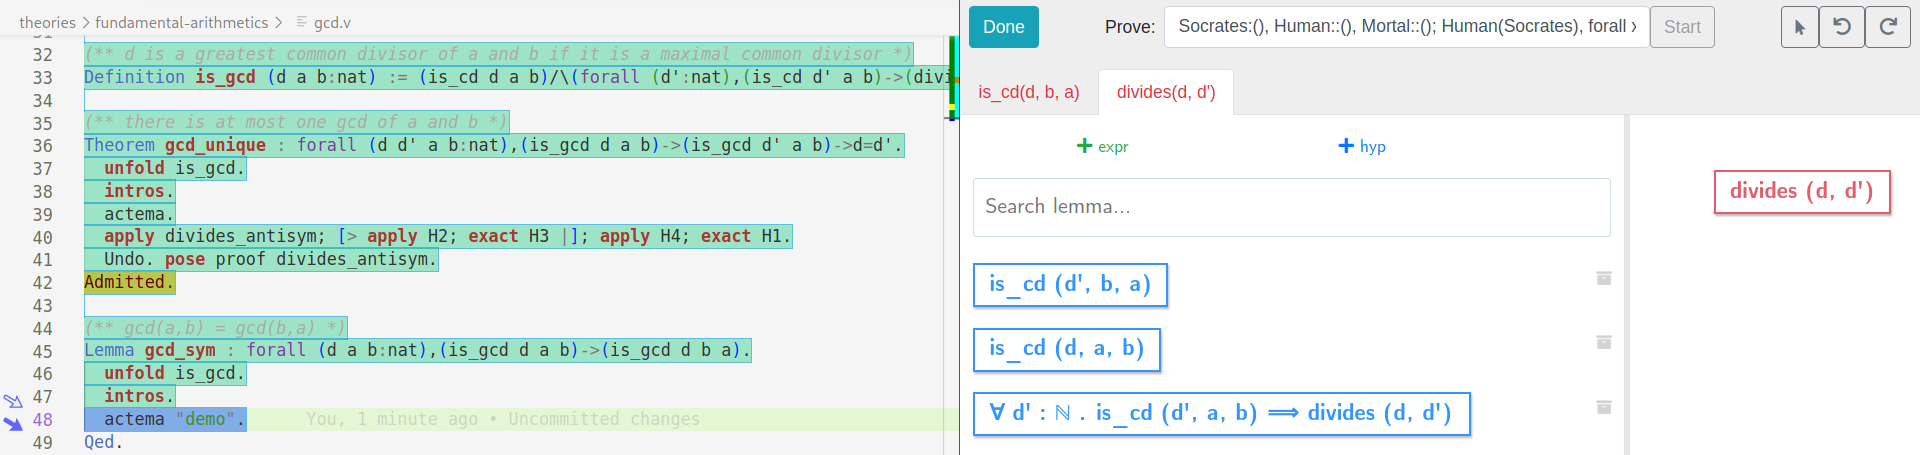
\includegraphics[width=1.5\textwidth]{coq-actema.png}
  \AP On the left, the usual interactive view of the \kl{proof script}, in the
  \intro{VsCoq} \kl{IDE} \cite{VsCoq}. On the right, the graphical \kl{proof view} of
  \kl{Actema}.
  \caption{ Graphical layout of the \kl{coq-actema} system}
  \labfig{coq-actema}
\end{figure*}

Let us now give the full picture of the \kl{coq-actema} system that integrates
both \kl{Actema} and the \kl{Coq} plugin. A schematic view of its overall
architecture, including the various components and their relationships, is
provided in \reffig{archi}. The different \emph{processes/agents} involved are
represented by shapes of different \emph{colors}, and we add a directed
\emph{arrow} whenever two of them communicate with each other, where the
\emph{source} requests data from or sends instructions to the \emph{target}.

The \process{User} (pink circle) is the only human agent in the system, and
drives all interactions. She interacts with the \kl{Coq} and \kl{Actema}
subsystems (transparent rectangles), through the interfaces provided by her
\kl{Coq} \process{IDE} of choice (blue rectangle) and \kl{Actema}'s
\process{Frontend} (yellow rectangle). This will typically take the form of a
two-windows layout, as depicted by the screenshot of \reffig{coq-actema}.

\subsection{Actema web app}

\AP
The \kl{Actema} web app runs in a process independent from \kl{Coq}, represented
by the yellow \process{Interface} rectangle. We add a third layer to the
\process{Frontend} and \process{Backend} described in \refsec{actema}, namely a
\intro{HTTP} \process{Server} (orange rectangle) that handles requests from, and
responses to the \kl{Coq} \process{Plugin}. Thus we implement interprocess
communication between \kl{Actema} and \kl{Coq} through the network layer of the
operating system, rather than a more local mechanism such as Unix pipelines.
There are a few reasons behind our choice of the \kl{HTTP} protocol:
\begin{itemize}
  \item it provides useful abstractions when working with a client/server
    architecture structured around requests;
  \item it is a widely spread standard, especially in web technologies. Thus we
    were able to reduce development time by reusing generic implementations of
    both client and server from standard libraries;
  \item more anecdotically, this makes it easy to run \kl{Coq} and \kl{Actema}
    on different machines connected on the same network. This could be used for
    instance to offload heavy computations in a proof to the machine running
    \kl{Coq}, while still being able to interact with \kl{Coq} through
    \kl{Actema} on the weaker machine.
\end{itemize}
The \process{Server} runs in a process separate from the \process{Interface}, in
order to avoid any delay in the latter. Then we bundle everything in an
\intro{Electron} application \cite{Electron}, so that \kl{Actema} can easily be
run locally on most operating systems. This also allows us to exploit the
multi-process architecture of Electron \cite{ElectronProcess}, where the
so-called \emph{main} process runs the server and has the ability to issue
system calls for networking through the \intro{Node.js} \kl{HTTP} library
\cite{NodeJS}; and the so-called \emph{renderer} process runs the
\process{Interface} in the \intro{Chromium} browser.

\subsection{Coq plugin}

The \process{Plugin} is loaded dynamically in \kl{Coq}'s \process{Engine} (green
rectangle) by executing the following command in a \kl{proof script}:
\begin{minted}[fontsize=\normalsize]{coq}
  From Actema Require Import Loader.
\end{minted}
% This can be done dynamically by the \process{User} in her \process{IDE}, or
% statically at compile time.
It exposes a single \kl{tactic} called \texttt{actema}, which can run in two
distinct modes:
\begin{description}
  \item[\bfseries Interactive] The \process{Plugin} sends the current
  \kl{subgoal}s to \kl{Actema}, and the user applies a sequence of \kl{actions} on
  them. Each time an \kl{action} is performed, it is sent back to \kl{Coq}, compiled
  into the appropriate \kl{tactic} call, and then executed to generate new
  \kl{subgoals} that are sent again to \kl{Actema}. The \texttt{actema}
  \kl{tactic} finishes its execution either when:
  \begin{itemize}
    \item all \kl{subgoals} are proved (in \kl{Actema});
    \item the \process{User} decides to stop and give back control to the
    \process{IDE};
    \item in some rare cases, an unrecoverable error occurs.
  \end{itemize}

  \item[\bfseries Non-interactive] If the \texttt{actema} \kl{tactic} has
  already been executed on the \kl{subgoal} under focus, then the
  \process{Plugin} automatically saved the sequence of \kl{actions} performed by the
  \process{User} in a \process{Database} (gray circle). Currently for ease of
  development, the \process{Database} is implemented as a simple directory on
  the local filesystem, where each file encodes an entry as follows:
  \begin{itemize}
    \item the filename is a hash code that uniquely identifies the \kl{goal} by both
    its \emph{content}, i.e. the statements of the hypotheses and conclusion,
    and an optional \emph{identifier}, which can be given as argument to the
    \kl{tactic} in the form of an arbitrary string;
    \item the contents of the file is a \intro{Base64} encoding of
    the data specifying each \kl{action}, whose format will be detailed in
    \refsec{compilation}.
  \end{itemize}
  Then the \kl{tactic} will load the sequence of \kl{actions} from the appropriate file,
  recompile it into one big \kl{tactic}, and execute it on the current \kl{subgoal}.
\end{description}
One can also force the execution in interactive mode by using a variant of the
tactic named \texttt{actema\_force}. We provide details of the complete
interaction protocol followed by the \texttt{actema} \kl{tactic} in the following
section.

\AP
Regarding the implementation of the \process{Plugin}, we chose to do it in the
standard way by interfacing with the \intro{coq-core} API in \kl{OCaml}
\cite{CoqCore}, although it has been encouraged in recent versions of \kl{Coq}
to interface with more stable APIs such as those provided by \intro{Coq-Elpi}
\cite{CoqELPI} and \intro{MetaCoq} \sidecite{MetaCoq}\sidenote{Indeed, breaking
changes are frequently introduced in \kl{coq-core} with newer versions of
\kl{Coq}, which requires more maintenance efforts from plugin developers.}. The
main reason is that our plugin performs \emph{side effects} by interacting with
an external environment: the file system when saving and retrieving graphical
proofs, and the network when issueing \kl{HTTP} requests to \kl{Actema}. Those
cannot be implemented in the aforementioned frameworks.

\section{Interaction protocol}\labsec{protocol}

\begin{figure*}
  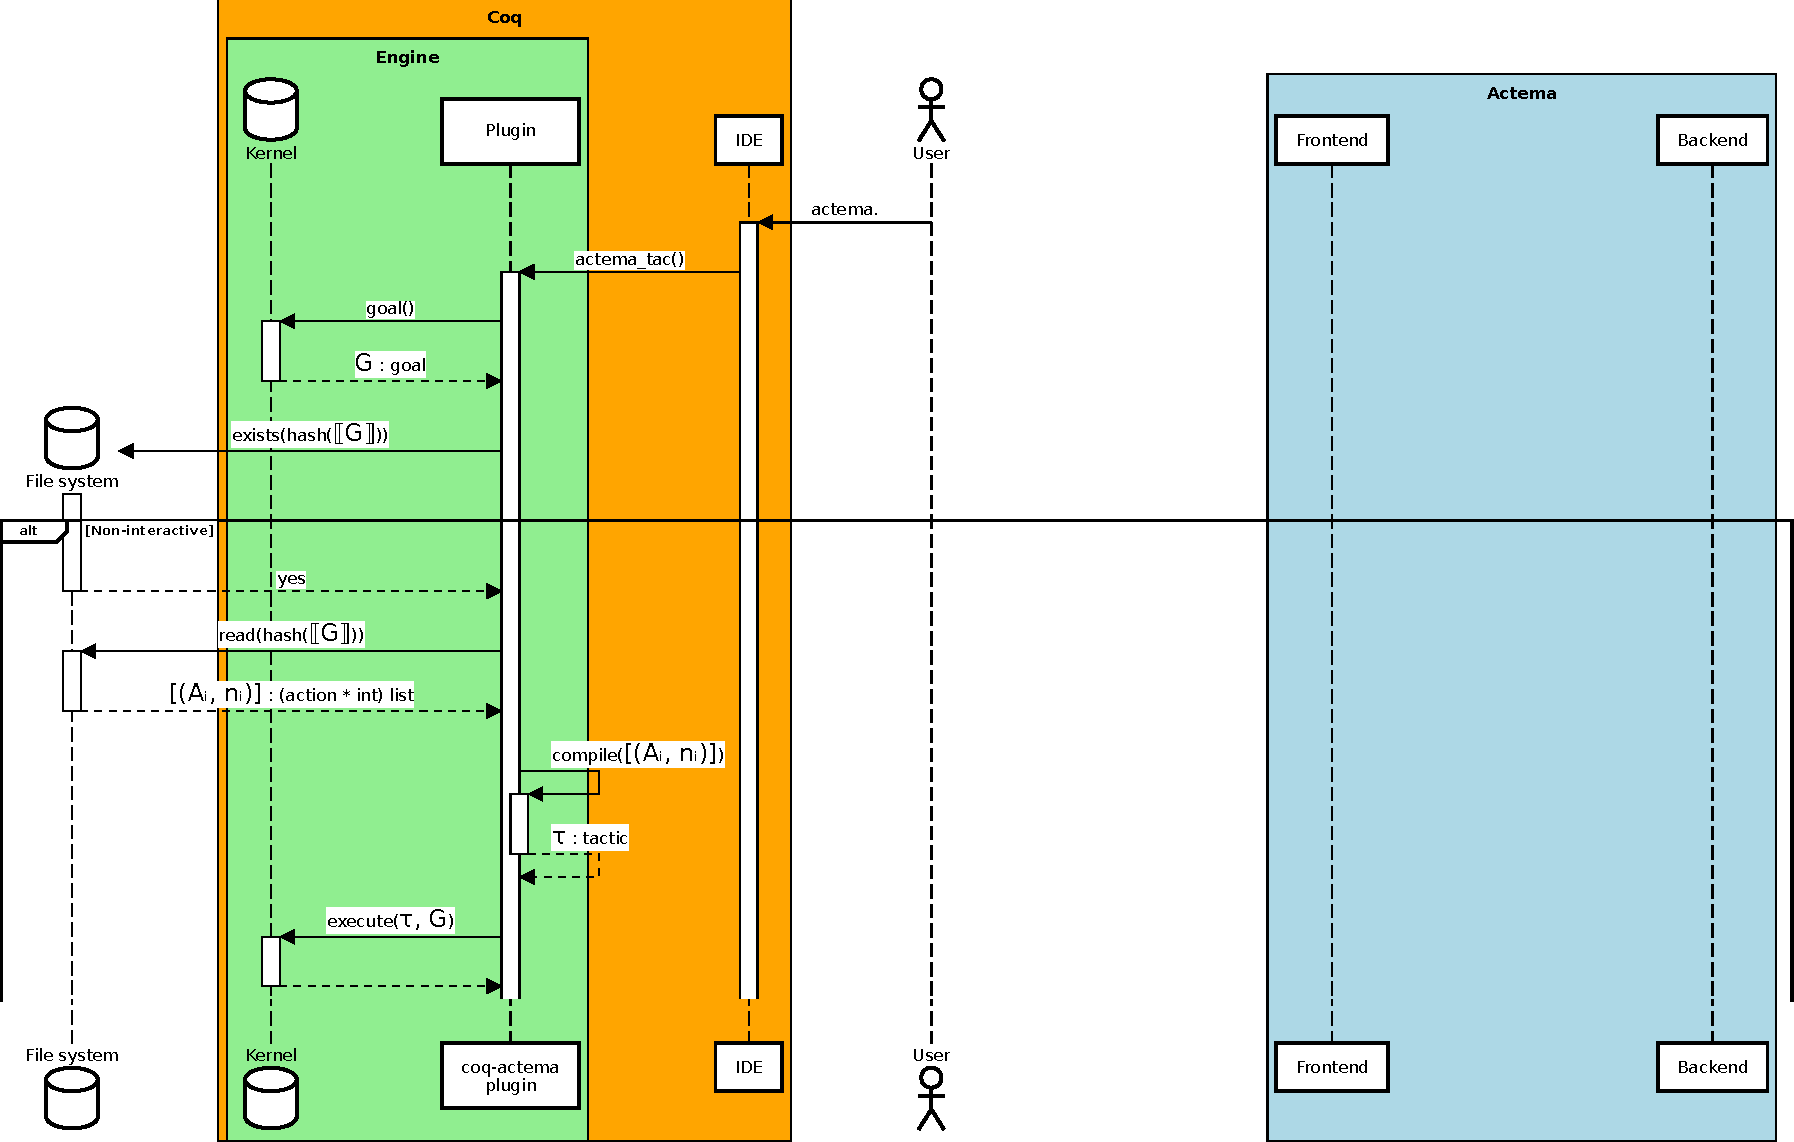
\includegraphics[angle=90,height=\textheight]{protocol-1.pdf}
  \vspace{2em}
  \caption{Sequence diagram of \kl{coq-actema}'s interaction protocol ---
  non-interactive mode}
  \labfig{protocol1}
\end{figure*}

\begin{figure*}
  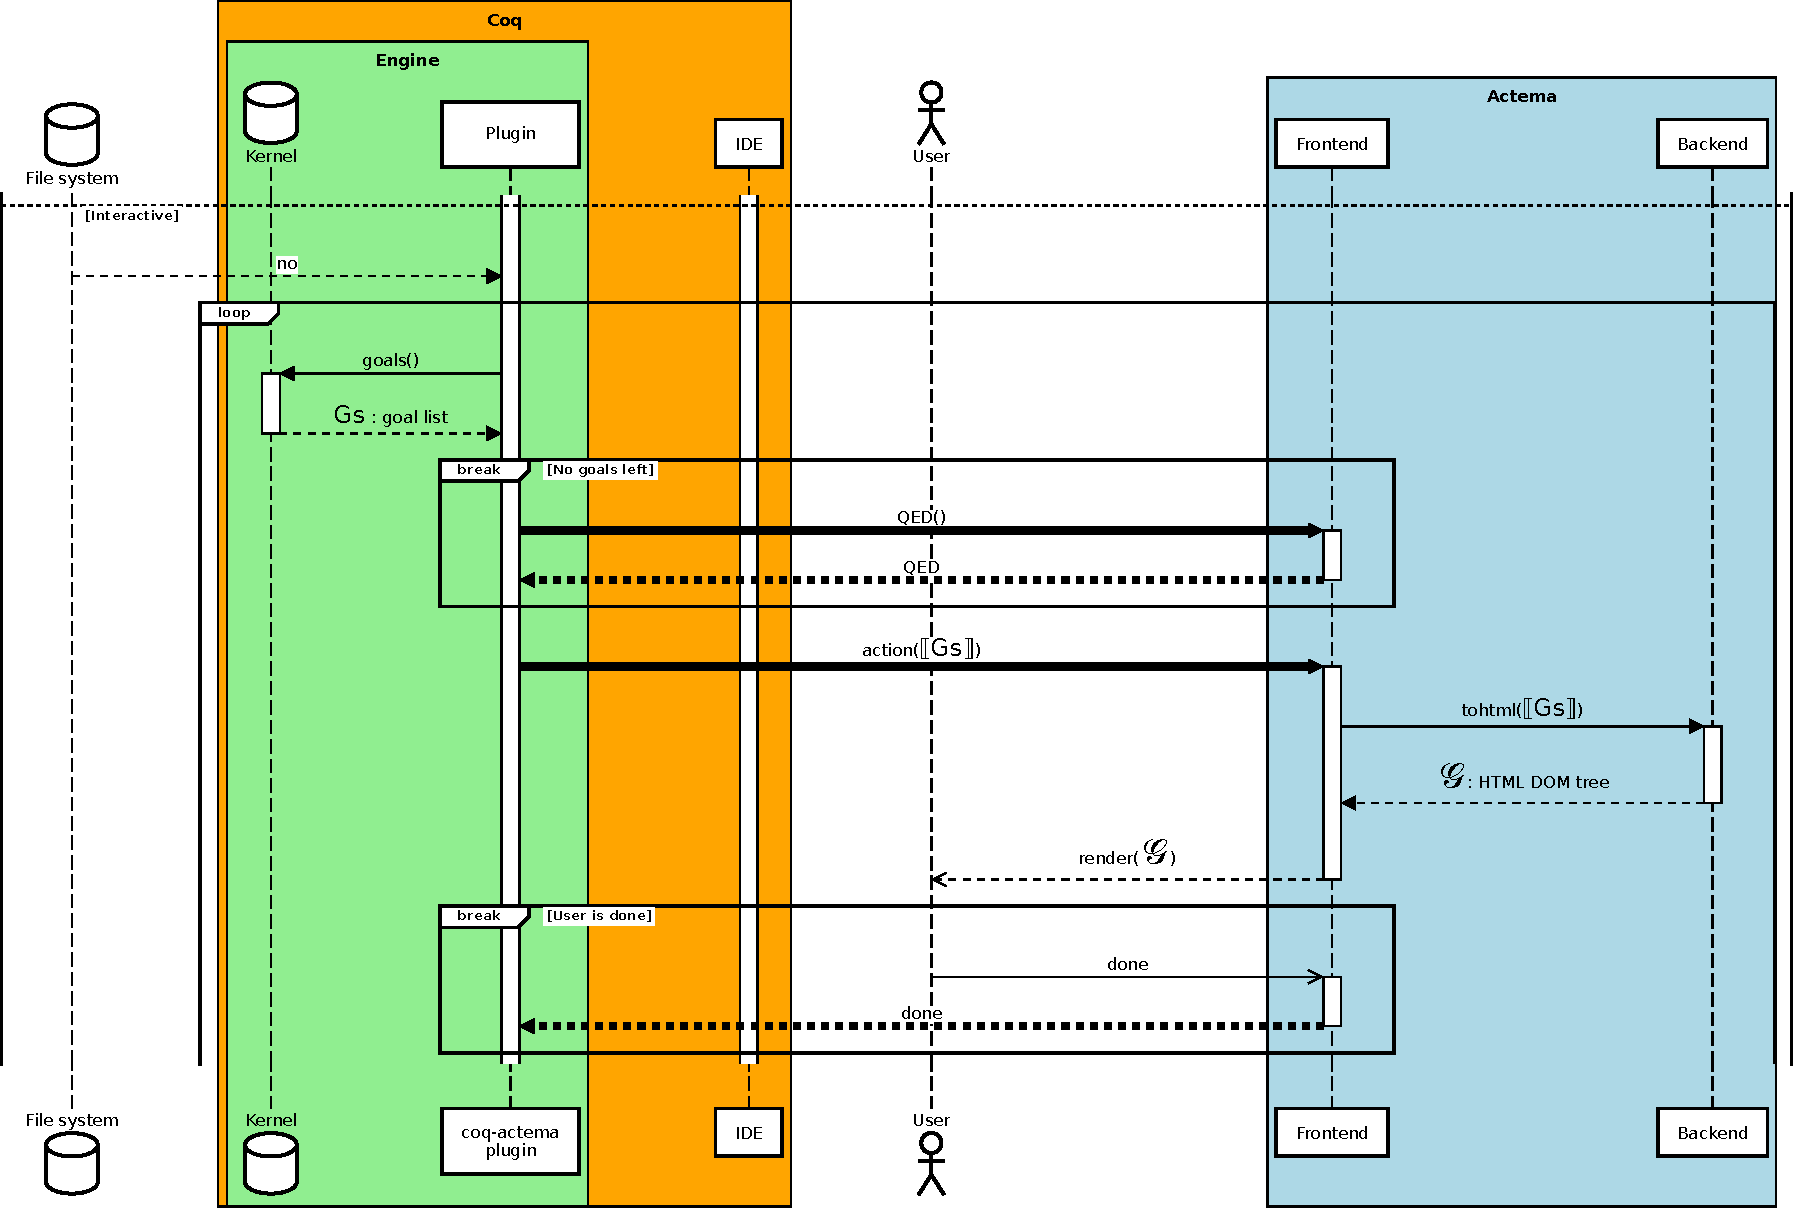
\includegraphics[angle=90,height=\textheight]{protocol-2.pdf}
  \vspace{2em}
  \caption{Sequence diagram of \kl{coq-actema}'s interaction protocol ---
    breaking out of the interaction loop}
  \labfig{protocol2}
\end{figure*}

\begin{figure*}
  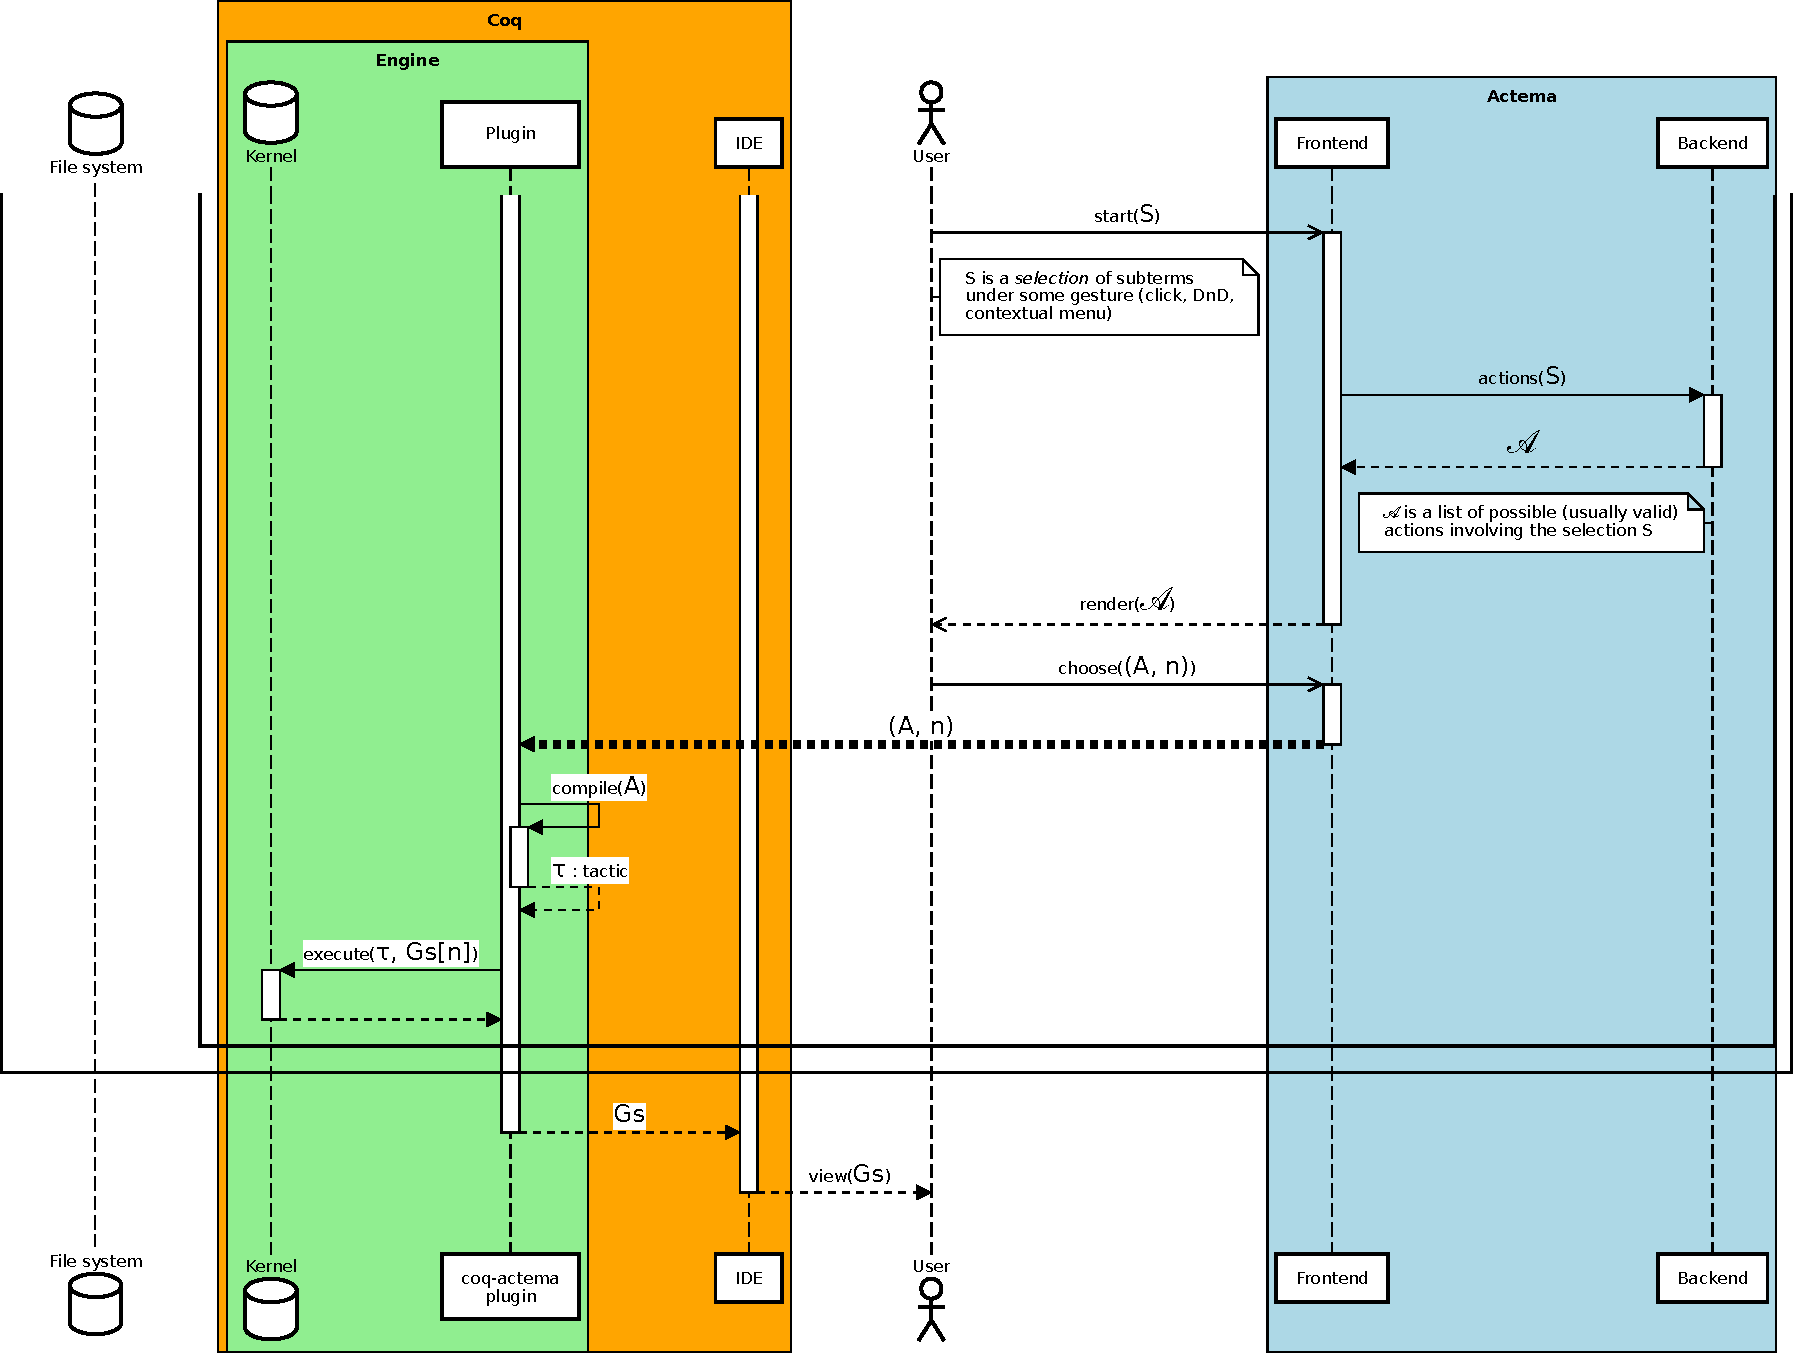
\includegraphics[angle=90,height=0.9\textheight]{protocol-3.pdf}
  \vspace{2em}
  \caption{Sequence diagram of \kl{coq-actema}'s interaction protocol ---
    applying an action}
  \labfig{protocol3}
\end{figure*}

\AP
We will now unroll the details of a complete interaction in \kl{coq-actema},
starting from the \process{User} calling the \texttt{actema} \kl{tactic} in her
\process{IDE}, and ending with her viewing the new \kl{subgoals} displayed in
the \process{IDE}. We chose to represent this with a \intro{sequence diagram},
as specified by the \intro{UML} standard \cite{enwiki:1153944336}. This kind of
\kl{diagram} is used to depict runtime behavior of a system, showing
interactions between objects and the messages they exchange in the order they
occur chronologically. In our case, the objects are the different processes
described in the previous section, as well as the \process{User}. Since the full
interaction is quite involved, we split the \kl{diagram} in three parts:
\reffig{protocol1} includes the beginning of the interaction, focusing on the
non-interactive mode of the \texttt{actema} \kl{tactic} where the
\process{Plugin} communicates with \kl{Coq}'s \kl(PA){kernel} and the
\process{Database}. \reffig{protocol2} and \reffig{protocol3} tackle the
interactive mode of the \texttt{actema} \kl{tactic}: \reffig{protocol2} focuses
on the conditions for breaking out of the interaction loop, and
\reffig{protocol3} on the interactions at work when the \process{User} performs
a proof \kl{action} in \kl{Actema}.

\subsection{Translating goals}

\AP
The first task performed by the \process{Plugin} when calling the
\texttt{actema} \kl{tactic} is to ask the \kl(PA){kernel} for the data of the
\kl{subgoal} $G$ currently under focus. Then for the \kl{goal} $G$ to be
understandable by the \process{Backend} of \kl{Actema}, the \process{Plugin}
will translate it into a new representation $\intro*\trgoal{G}$ in a custom datatype.
In order to share the definition of this datatype across implementations of the
\process{Plugin} and \process{Backend}, we decided to use the \intro{ATD} data
specification language \cite{ATD}. It provides a set of tools to automatically
generate idiomatic datatype definitions in a few target languages --- including
\kl{OCaml} --- along with (de)serialization and validation helpers. This is
particularly fit for our usecase, where we need to serialize complex data like
$\trgoal{G}$ in order to transmit it over \kl{HTTP} messages. Since both the
\process{Plugin} and \process{Backend} are written in \kl{OCaml}, it also allows
us to share across implementations our own domain-specific helpers for
manipulating this data.

\begin{figure}
  \begin{minted}
  [
  frame=lines,
  framesep=2mm,
  baselinestretch=1,
  fontsize=\footnotesize,
  linenos
  ]
  {ocaml}

(* -------------------------------------------------------------------- *)
(** Identifiers *)

type name = string

(* -------------------------------------------------------------------- *)
(** Types *)

type type_ = [
  | TVar of name
]

type arity = type_ list
type sig_  = (arity * type_)

(* -------------------------------------------------------------------- *)
(** Expressions *)

type expr = [
  | EVar of name
  | EFun of (name * expr list)
]

(* -------------------------------------------------------------------- *)
(** Formulas *)

type logcon = [ And | Or | Imp | Equiv | Not ]
type bkind  = [ Forall | Exist ]

type form = [
  | FTrue
  | FFalse
  | FPred of (name * expr list)
  | FConn of (logcon * form list)
  | FBind of (bkind * name * type_ * form)
]

(* -------------------------------------------------------------------- *)
(** Terms = Formulas + Expressions *)

type term = [F of form | E of expr]

(* -------------------------------------------------------------------- *)
(** Environments *)

(* Body of a variable declaration, holding its type and eventually an expression
    in the case of a local definition *)
type bvar = (type_ * expr option)

type varenv = (name * bvar) list

type env = {
  env_sort      : name                       list; (* Sorts, i.e. atomic types *)
  env_prp       : (name * arity            ) list; (* Predicate symbols *)
  env_fun       : (name * sig_             ) list; (* Function symbols *)
  env_sort_name : (name * name             ) list;
  env_prp_name  : (name * name             ) list;
  env_fun_name  : (name * name             ) list;
  env_var       : varenv;                          (* Variable declarations *)
}

(* Local environment, only maps abstract variables to their type *)
type lenv = (name * type_) list 

\end{minted}

  \caption{\kl{ATD} definitions for \kl{first-order} formulas and environments}
  \labfig{atd-fo}
\end{figure}

\begin{figure}
  \begin{minted}
  [
  frame=lines,
  framesep=2mm,
  baselinestretch=1,
  fontsize=\footnotesize,
  linenos
  ]
  {ocaml}

(* -------------------------------------------------------------------- *)
(** Goals *)

(* Unique identifier *)
type uid = string

(* Hypothesis *)
type hyp = {
  h_id : uid;
  h_form : form;
}

(* Goal *)
type goal = {
  g_env : env;
  g_hyps : hyp list;
  g_concl : form;
}

type goals = goal list

(* Abstract goal, without the signature *)
type agoal = {
  a_vars : varenv;
  a_hyps : hyp list;
  a_concl : form;
}

\end{minted}

  \caption{\kl{ATD} definitions for \kl{goals}}
  \labfig{atd-goals}
\end{figure}

The \kl{ATD} definition of \kl{goals} is given by the \texttt{goal} type in
\reffig{atd-goals}\sidenote{The syntax is almost the same as that of \kl{OCaml}
datatypes, for the reader already acquainted with this language.}. It relies on
the \kl{ATD} types \texttt{form} of \emph{formulas}, and \texttt{env} of
\emph{environments} of available constants and variables. In our setting, these
correspond respectively to the formulas and \emph{signatures} of many-sorted
\kl{FOL}, whose \kl{ATD} definitions are given in \reffig{atd-fo}. But
one could imagine using formulas and environments in \kl{higher-order} logic
instead, and this would not change the structure of the \texttt{goal} datatype.
Note that hypotheses are encoded with a \texttt{h\_id} attribute corresponding
to their string identifier in the \kl{Coq} \kl{goal}, even though we do not
display it in \kl{Actema}'s interface. This is required later by the plugin to
compile \kl{actions} into \kl{tactics}, because we need to identify which \kl{Coq}
hypotheses correspond to those designated graphically by the \process{User}.

\subsection{Retrieving actions}

\AP
The next step for the \process{Plugin} is to check if there already exists a
graphical proof associated to $\trgoal{G}$ in the \process{Database}. If so,
then it retrieves it in the form of a list $A$ of \emph{actions}, whose data
format will be precised in \refsec{compilation}. There is also a positive
integer $n_i$ associated to each \kl{action} $A_i$ in the list, corresponding to the
index of the \kl{goal} to which $A_i$ applies in the list of \kl{subgoals}. Then
each $A_i$ is compiled into a \kl{tactic} $\intro*\traction{A_i}$, and all the
$\traction{A_i}$ are composed into a unique \kl{tactic} $\tau$, which is
executed by the \kl(PA){kernel} on $G$ to apply the full sequence of \kl{actions}.

\begin{remark}
  Currently the translation $\trgoal{-}$ is not \emph{injective}: it might
  map two different \kl{Coq} \kl{goals} to the same \kl{Actema} \kl{goal},
  because strictly \kl{higher-order} subterms are translated into a
  \texttt{dummy} atomic predicate/function. Thus one might retrieve a proof from
  a different \kl{goal} when calling the \texttt{actema} \kl{tactic}. However
  this is not problematic, since the \process{User} cannot perform any \kl{actions}
  involving the parts of the two goals that make them distinct; they might as
  well be seen as the same \kl{goal} from her point of view. It can thus be
  considered as a feature that maximizes proof reuse.
\end{remark}

If there is no saved proof for $\trgoal{G}$, then the \texttt{actema}
\kl{tactic} has never been executed on $\trgoal{G}$, and thus we let the
\process{User} provide a (partial) proof in \kl{Actema}. First the
\process{Plugin} retrieves the list $Gs$ of all \kl{subgoals}, instead of just
the one under focus. If $Gs$ is empty, which would happen after all subgoals
have been solved from \kl{Actema}, then it sends a \request{QED} request to
\kl{Actema} so that the latter can update its view accordingly, and the
interaction loop with \kl{Actema} stops here\sidenote{In \reffig{protocol2} and
\reffig{protocol3}, we depict requests as being sent to the \process{Frontend}
of \kl{Actema}. This is an imprecision for trading in some readability, since as
reviewed in \refsec{architecture} it is the \process{Server} which handles
communication with the \process{Plugin}, and in particular forwards requests to
the \process{Frontend}.}.

\AP
If $Gs$ is not empty then there is at least one \kl{subgoal}, and we send an
\request{action} \kl{HTTP} request to \kl{Actema}, whose body contains the
translated \kl{subgoals} $\trgoal{Gs}$. To do this, we chose to serialize
$\trgoal{Gs}$ with the \intro{Biniou} helpers autogenerated by \intro{atdgen},
the \kl{OCaml} backend of \kl{ATD}. According to its authors: ``Biniou is a
binary format extensible like JSON but more compact and faster to process''
\cite{atdgen}. This data is then deserialized and compiled into a set
$\mathcal{G}$ of \kl{HTML} \intro{DOM} nodes by the \process{Backend}, so that
the goals can be rendered by the \process{Frontend} and exposed to the
\process{User}. Then the \process{User} has two options:
\begin{itemize}
  \item she can apply either a click, \kl{DnD} or \kl{contextual
  action}\sidenote{See \refsec{funcs} for an introductory example of
  \kl{contextual action} with \kl{Unfold}.}. The precise protocol followed for
  applying an \kl{action} is summarized in \reftab{action-protocol}. Let us focus on
  the more complex case of \kl{DnD} \kl{actions}. The \textbf{Start} column describes
  how the \process{User} \emph{starts} the \kl{action}, here by dragging some
  \kl{item} $I$ of the current \kl{subgoal}. Then the \process{Frontend} asks
  the \process{Backend} for the set $\mathcal{A}$ of all available \kl{DnD}
  \kl{actions} involving $I$. The \textbf{Selection} column describes how the
  computation of $\mathcal{A}$ is impacted by the set $S$ of subterms that are
  selected in the current \kl{subgoal}. For \kl{DnD} \kl{actions}, we essentially
  filter out all \kl{linkages} that do not match the selection. The
  \textbf{Render} column describes how $\mathcal{A}$ is \emph{rendered} to the
  \process{User}: here we highlight the set $Q$ of all \kl(sfl){valid} drop
  targets, which correspond to subterms of the current \kl{goal} located in
  other \kl{items}\sidenote{Highlighting is here understood in a \emph{visual}
  sense: in the current implementation of \kl{Actema}, subterms are indicated
  graphically by squaring them. But one could imagine other modalities for
  highlighting, typically \emph{spelling} the subterms with a speech synthesis
  algorithm, e.g. for users with impaired vision.}. Lastly, the \textbf{End}
  column describes how the user chooses a specific \kl{action} $A \in \mathcal{A}$ to
  apply, here by dropping $I$ on a given target $q$. Then $A$ is serialized and
  sent in the body of the response to the \request{action} request, together
  with the index $n$ of the \kl{subgoal} under focus in \kl{Actema}. The
  \process{Plugin} can therefore compile $A$ into a \kl{tactic} $\traction{A}$
  which is executed on the $n^{\text{th}}$ Coq \kl{subgoal}, giving a new list
  of \kl{subgoals} which is sent again to \kl{Actema} for another round of the
  interaction loop.

  \item or she can click on a \texttt{Done} button in \kl{Actema}'s interface:
  this has the effect of answering the \request{action} request from the
  \process{Plugin} with a \request{done} response, and the interaction loop with
  \kl{Actema} stops here. This will happen when the \process{User} wants to go
  back to editing the \kl{proof script}, either because she is satisfied with
  the new \kl{subgoals} obtained from previous \kl{actions}, or because she is stuck
  and wants to try native \kl{Coq} \kl{tactics} instead. Indeed our protocol is
  \emph{synchronous}: the \process{IDE}'s interface is stuck until the
  \texttt{actema} \kl{tactic} has finished its execution, and thus one cannot
  edit the \kl{proof script} \emph{and} build a proof in \kl{Actema} at the same
  time.
  % \sidenote{This is because the
  % \emph{document checking model} of most \kl{Coq} IDEs is itself synchronous: when
  % the \process{User} modifies the \kl{proof script} at a location before the current
  % execution point, the proof state goes back to how it was at that location, and
  % every command/tactic coming after it needs to be reinterpreted.}
\end{itemize}

\begin{table*}[]
  \def\arraystretch{1.5}
  \begin{tabular}{|c|C{0.2\textwidth}|C{0.4\textwidth}|C{0.25\textwidth}|C{0.2\textwidth}|}
  \hline
  \textbf{Kind} & \textbf{Start}       & \textbf{Selection $S$} &
  \textbf{Render}                      & \textbf{End} \\ \hline
  Click         & Hover \kl{item} $I$       & Ignored & Highlight $P \subseteq
  \subterms{I}$ & Click on some $p \in P$    \\ \hline
  \kl{DnD}           & Drag \kl{item} $I$        &
      If $\exists p \in S \cap \subterms{I}$ then match only $p \link q$ where
      $q \in \substermscompl{\subterms{I}}$
      \newline
      If $\exists q \in S \cap \substermscompl{\subterms{I}}$ then match only $p
      \link q$ where $p \in \subterms{I}$
    & Highlight $Q \subseteq \substermscompl{\subterms{I}}$ & Drop on some $q \in Q$ \\ \hline
  Contextual    & Open menu & Populate menu only with \kl{actions}
  applicable on $S$ & Show menu & Choose an \kl{item} in the menu \\ \hline
  \end{tabular}
  \raggedright
  \parbox{\textwidth}{
    \vspace{1.5em}
    We introduced some notations for conciseness:
    \begin{itemize}
      \item $p, q$ denote \kl{paths} to subterms of the current goal
      \item $P, Q$ and the selection $S$ denote sets of \kl{paths}
      \item $\intro*\subterms{I}$ denotes the set of \kl{paths} within \kl{item} $I$
      \item $\substermscompl{\subterms{I}}$ denotes the complement of $\subterms{I}$, i.e.
      all \kl{paths} in all \kl{items} $J \not= I$
      \item $p @ q$ is a \kl{linkage} as introduced in \refsec{linkages}
    \end{itemize}}

  \caption{Protocol for applying an \kl{action} in Actema}
  \labtab{action-protocol}
\end{table*}


\section{Compiling actions}\labsec{compilation}

Once the \process{Plugin} has received the \kl{actions} to execute, either from the
\process{Database} or the \process{User}, it will compile them with the function
$\traction{-}$ which translates any \kl{action} $A$ into a \kl{Coq} tactic
$\traction{A}$. This function actually has access to some other data: \kl{Coq}'s
\kl{goal} $G$, its \kl{Actema} translation $\trgoal{G}$, and a bijective mapping
$\Sigma$ between \kl{Coq} constants in the environment of $G$ and the
corresponding \kl{Actema} symbols in the \kl{first-order} signature of
$\trgoal{G}$.

\subsection{The \texttt{action} datatype}

\begin{figure}
  \begin{minted}
  [
  frame=lines,
  framesep=2mm,
  baselinestretch=1,
  fontsize=\footnotesize,
  linenos
  ]
  {ocaml}
  
(* -------------------------------------------------------------------- *)
(** Actions *)

(* A path refers to a subterm in the current subgoal, through a [handle]
    identifying an item of kind [kind], and a list of integers [sub] designating
    the specific subterm of the item *)
type pkind = [Hyp | Concl | Var of [Head | Body]]
type ctxt = { kind : pkind; handle : uid }
type ipath = { ctxt : ctxt; sub : int list }

(* Trace of a subformula linking, from which the list of rewrite rules to apply
   can be reconstructed *)
type choice = (int * (lenv * lenv * expr) option)
type itrace = choice list

type action = [
  | AId                                     (* The empty action which does nothing *)
  | ADef of (name * type_ * expr)           (* Introduction of a local definition *)
  | AIntro of (int * (expr * type_) option) (* Click on a conclusion *)
  | AExact of uid                           (* Proof by assumption *)
  | AElim of (uid * int)                    (* Click on a hypothesis *)
  | AInd of uid                             (* Click on a variable of inductive type *)
  | ASimpl of ipath                         (* Simplify contextual action *)
  | ARed of ipath                           (* Unfold contextual action *)
  | AIndt of ipath                          (* Induction contextual action *)
  | APbp of ipath                           (* Proof-by-Pointing contextual action *)
  | ACase of ipath                          (* Case contextual action *)
  | ACut of form                            (* Click on +hyp button *)
  | AGeneralize of uid                      (* Generalization of a hypothesis *)
  | AMove of (uid * uid option)             (* Reordering of a hypothesis *)
  | ADuplicate of uid                       (* Duplication of a hypothesis *)
  | ALink of (ipath * ipath * itrace)       (* DnD action for subformula linking *)
  | AInstantiate of (expr * ipath)          (* DnD action for instantiating a quantifier *)
]

(* An action identifier is a pair of an abstract goal and an arbitrary string identifier *)
type aident = (string * agoal)

\end{minted}

  \caption{\kl{ATD} definitions for actions}
  \labfig{atd-actions}
\end{figure}

The \texttt{action} datatype is described thoroughly in the \kl{ATD} specification
provided in \reffig{atd-actions}. It is a big algebraic datatype, where each
constructor encodes a specific \emph{type} of \kl{action}. An action's type is
equivalent to the \emph{signature} of a \kl{tactic}, i.e. its name and the types
of its arguments. In particular, the translation function $\traction{-}$ is
defined as a big pattern-matching on the action's type\sidenote{Note that an
action's type is orthogonal to what we referred to as its \emph{kind} in
\reftab{action-protocol}, that is the interface mechanism through which it is
accessible. One might for example want to map some \kl{action} types to \emph{vocal
commands} instead of click or \kl{DnD} gestures.}. The arguments in \kl{action} types
rely on most datatypes defined previously in \reffig{atd-fo} and
\reffig{atd-goals}, and on two new datatypes: the type \texttt{ipath} of
\emph{\kl{paths}}, which is used pervasively to designate subterms of the current
\kl{subgoal} (that are typically indicated by the \process{User} through
pointing); and the type \texttt{itrace} of \emph{\kl{subformula linking}
traces}, which is used in the compilation of \kl{DnD} \kl{actions} that perform
\kl{subformula linking}, to be described soon.

Most click and \kl{contextual actions} have a straightforward translation as \kl{Coq}
tactics. For instance, the \texttt{AIntro} \kl{action} that corresponds to a click on
the conclusion $C$ will be mapped to the \kl{Coq} \kl{tactic} that introduces
the main connective of $C$, and is thus defined by case on the latter:
\texttt{intro} for $\limp$ and $\forall$, \texttt{split} for $\land$, etc. The
\kl{actions} \texttt{AInd}, \texttt{ASimpl} and \texttt{ARed} correspond respectively
to the \kl{contextual actions} \kl{Induction}, \kl{Simplify} and
\kl{Unfold} introduced in \refch{advanced}, and are mapped almost directly
to the equivalent \kl{Coq} \kl{tactics} \texttt{induction}, \texttt{simpl} and
\texttt{red}. The only difference is that they have a \emph{\kl{deep inference}}
flavor, since they can all be applied on an arbitrary subterm selected by the
\process{User}. This relies on our implementation of \kl{deep inference}
semantics directly in \kl{Coq}, that we now briefly describe.

\subsection{Deep inference semantics}

\AP
In a \kl{deep inference} setting, one can reason on subterms located arbitrarily
\emph{deep} inside statements, usually by applying some kind of \kl{rewriting
rules} on them. In particular, the semantics of \kl{DnD} \kl{actions} described in
\refch{sfl} are based on the rules of \kl{SFL} (\reffig{DISL}). To implement
them, we chose to do a \intro{deep embedding} of \kl{FOL} inside \kl{CoIC}. Here
the word ``deep'' has a different meaning, related to the fact that we encode
the statements of \kl{FOL} with our own custom datatypes, instead of reusing the
statements of \kl{CoIC}. This makes it easier to define the \kl{SFL}
\kl{rewriting rules}, in particular because we need to manipulate
\emph{\kl{contexts}} (\refdef{formula-context}) explicitly, and those are not
available for \kl{CoIC} propositions.

\AP
Then we use a technique called \intro{computational reflection} in order to
apply the embedded \kl{deep inference} semantics to \kl{Coq} \kl{goals}.
Originating from the \emph{small scale reflection} methodology supported by the
{\kl{\ssreflect}} framework \cite{SSR}, it consists in:
\begin{enumerate}
  \item translating \kl{Coq} objects into their equivalent formulation in the
\kl{deep embedding} with a \texttt{reify} function;
  \item reasoning on the \kl{deep embedding} with the help of \kl{Coq} programs
(also called \emph{fixpoints});
  \item translating objects back into \kl{Coq} with a \texttt{reflect} function.
\end{enumerate}
\AP
It is easy to implement the \texttt{reflect} function because the datatypes in a
\kl{deep embedding} are almost always defined as \emph{inductive} \kl{types},
and thus one can easily do pattern-matching on them. It is a different story for
the \texttt{reify} function, especially in our case: indeed we want to translate
the statements of \kl{Coq} \kl{goals} into \kl{first-order} propositions. But
\kl{Coq} statements are objects of \kl{type} \texttt{Prop}, and thus cannot be
pattern-matched on inside \kl{CoIC}\sidenote{For reasons of \kl{consistency} of
the logic, well-known in the literature on \kl{type theory}.}. Thus we need to
have recourse to a \emph{meta-programming} language in order to inspect the
structure of \kl{Coq} \kl{goals}. Here we use the standard \intro{Ltac}
language, which provides powerful constructs for pattern-matching on
\kl{goals}\sidenote{A downside of \kl{Ltac} is that it is an \emph{untyped}
language, whose programs are notoriously hard to debug and maintain. One might
consider a cleaner implementation with more recent alternatives in the \kl{Coq}
ecosystem, such as the successor to \kl{Ltac} \intro{Ltac2} \cite{Ltac2}, or the
\kl{MetaCoq} project \cite{MetaCoq}.}.

The most complex \kl{tactics} are those implementing \kl(dnd){backward} and
\kl(dnd){forward} \kl{DnD} \kl{actions}, called respectively \texttt{backward} and
\texttt{forward}. They rely on two \kl{Coq} fixpoints \texttt{b3} and
\texttt{f3} which respectively compute the new conclusion $\mathtt{b3}(p, q, T)$
from a \kl(dnd){backward} \kl{linkage} $p \back q$, and the new hypothesis
$\mathtt{f3}(p, q, T)$ from a \kl(dnd){forward} \kl{linkage} $p \forw q$, where
$T$ is the so-called \emph{\kl{subformula linking} trace} mentioned earlier. Of
course the \kl{paths} $p, q$ and the trace $T$ are all expressed with custom
\kl{Coq} datatypes relying on our \kl{deep embedding} of \kl{FOL}. The role of
the trace in particular is to provide the list of \kl{SFL} \kl{rewriting rules}
to apply, as well as the \kl{Coq} \kl{terms} instantiating quantifiers that were
computed in \kl{Actema} by \kl{unification} of the two linked subformulas. Then
we formulate in \kl{Coq} two theorems that guarantee the logical
\emph{soundness} of \texttt{b3} and \texttt{f3} (\reffig{dnd-snd}),
corresponding to \refthm{sfl-soundness}. Note that the theorems are formulated
using the native implication connective \texttt{->} of \kl{Coq}, thanks to the
\texttt{reflect} function. The final \kl{tactics} \texttt{backward} and
\texttt{forward} can thus modify the \kl{goal} by applying these theorems, first
reifying the \kl{goal} with the \texttt{reify} function, and then relying on the
fact (also proved in \kl{Coq}) that \texttt{reflect} is the inverse of
\texttt{reify}.

\begin{figure}
  \begin{minted}
  [
  frame=lines,
  framesep=2mm,
  baselinestretch=1,
  fontsize=\footnotesize,
  linenos
  ]
  {coq}

Theorem b3_corr : forall p q T,
  coerce p -> coerce (b3 p q T) -> coerce q.

Theorem f3_corr : forall p q T,
  coerce p -> coerce q -> coerce (f3 p q T).

\end{minted}

  \caption{Soundness theorems of \kl{DnD} fixpoints in \kl{Coq}}
  \labfig{dnd-snd}
\end{figure}

% \begin{theorem}[Soundness of \kl{DnD} fixpoints]~\\
%   $$\forall p.\ \forall q.\ \forall T.\ \mathtt{reflect}(p) \limp
%   \mathtt{reflect}(\mathtt{b3}(p, q, T)) \limp \mathtt{reflect}(q)$$
%   \center{and}
%   $$\forall p.\ \forall q.\ \forall T.\ \mathtt{reflect}(p) \limp
%   \mathtt{reflect}(q) \limp \mathtt{reflect}(\mathtt{f3}(p, q, T))$$
% \end{theorem}

\begin{remark}
  There exist a few other approaches to the computer implementation of \kl{deep
  inference} systems. Ozan Kahramanoğulları has pioneered the field, by
  implementing various \kl{calculi of structures} inside frameworks like Maude
  \cite{kahramanogullari_maude_2008} and Tom
  \cite{kahramanogullari_implementing_2005} that are dedicated to the
  specification of \kl{rewriting systems}. For an integration within modern
  \kl{proof assistants}, we only know of Chaudhuri's recent work
  \sidecite{chaudhuri_certifying_2022} that explores different techniques in
  addition to reflection, like \emph{combinators} and some more powerful usages
  of \emph{metaprogramming}. He also provides an effective implementation of the
  techniques in his \kl{Profint} tool \cite{DBLP:conf/cade/Chaudhuri21}, that
  allows to export \kl{subformula linking} derivations built with \kl{Profint}'s
  \kl{GUI} as \kl{proof scripts} directly executable in various \kl{proof
  assistants} (\kl{Coq}, \kl{Lean}, \kl{Isabelle/HOL}).
\end{remark}

\section{Future works}\labsec{pluginfuture}

The \kl{coq-actema} system described in this chapter has been successfully
implemented and tested on various simple examples, including those of
\refsec{edukera} and \refsec{arith}. But there are many \kl{Coq} \kl{goals} that
cannot be properly handled in \kl{Actema}, which still hinders the usability of
the system in real mathematical developments, even in an educational setting.
Typically, the example of \refsec{funcs} cannot be completely performed in
\kl{Actema}, in this case because of the lack of support for
\emph{\kl{higher-order}} functions and predicates, but also because of the poor
support for user-defined \emph{notations}. Those are only a few of the current
limitations of \kl{coq-actema}, and we describe in the following pages how they
could be overcome, both to widen the scope and improve the \kl{UX} of the
system.

\subsection{Higher-order logic}

The importance of being able to express and manipulate \kl{higher-order}
functions and predicates has been stressed multiple times before. The fact that
\kl{Actema} is limited to \kl{first-order logic} is mostly a historical
contingency, motivated by the fact that some algorithms like \kl{unification}
are more tractable in this setting. But now that we rely on \kl{Coq}'s proof
engine, there is no fundamental reason for maintaining this choice. Because the
language of statements is at the foundation of a logical framework, many other
components of a \kl{proof assistant} will depend on it. Thus the switch to
\kl{higher-order} logic should be done as soon as possible, to limit the amount
of refactoring work to perform in the future. This will require changes to
\kl{Actema}'s \process{Backend} and \process{Frontend}, but also to the \kl{Coq}
\process{Plugin}\sidenote{The \kl{Coq} theory implementing the tactics for
\kl{deep inference}-based \kl{actions} already has partial support for
\kl{higher-order} \kl{goals}, thus work remains mostly on the side of the
translation module for \kl{Actema} written in \kl{OCaml}.} and the \kl{ATD}
datatype definitions enabling communication between the two.

One central question in the transition to \kl{higher-order} logic is how
\kl{unification} of subterms will be handled. Algorithms in this setting are
known to be incomplete because of undecidability
\sidecite{huet_undecidability_1973}, and their implementation can be very
tricky. The most sensible option seems to rely on the implementation already
provided by \kl{Coq}, which is the fruit of years of development and
improvements. But this would require changing the interaction protocol of
\kl{coq-actema}, by allowing the \process{Backend} of \kl{Actema} to make
\kl{unification} requests to the \process{Plugin}. This might be doable without
changing the current client-server architecture, but will probably involve some
intricate design decisions.

A more radical solution would be to replace the \request{actions} request from
the \process{Frontend} to the \process{Backend} by a \texttt{start} response
from the \process{Frontend} to the \process{Plugin}, with the data of the
selection in its body. Then we could completely delegate the computation of
available \kl{actions} to the \process{Plugin}, allowing us to freely use \kl{Coq}'s
\kl{unification}. This might not be too hard since we should be able to directly
reuse \kl{OCaml} code from the \process{Backend}, but is a deeper structural change
to the interaction protocol, that makes the \process{Plugin} responsible for an
important part of \kl{Actema}'s behavior. And this would induce a lot of
unnecessary reimplementation efforts if we were to port the \process{Plugin} to
other \kl{PAs}.

\subsection{Notations}

Another big limitation already mentioned in the introduction of this chapter, is
that we do not handle custom \emph{notations} for displaying
terms\sidenote{Apart from expressions in Peano arithmetic, for which we have ad
hoc support.}. It is however a crucial feature for making proofs in a specific
domain tractable, especially in the \kl{PbA} paradigm where one needs to
manipulate directly statements in the \kl{goal}. Now that we are connected to
\kl{Coq}, we can in principle reuse the notation system already implemented
within \kl{Coq}. The \kl{coq-core} \kl{OCaml} API indeed exposes methods for
pretty-printing \kl{Coq} terms using their assigned notations. The problem is
that these methods only return \emph{strings}, but in order to manipulate
\kl{terms} interactively in \kl{Actema} we also need access to \emph{trees}
mapping their subterm structure to the pretty-printed string. At the time of
writing there is no support for the latter, but the \kl{Coq} development team
informed us that they plan to add this feature. The same problem was met by the
developers of the \kl{ProofWidgets} framework in \kl{Lean}, and they had to
modify the pretty-printer of \kl{Lean} upstream\sidenote{Section 4.1 of
\cite{ayers_graphical_2021}.}.

Once one has support for custom notations displayed in an \kl{HTML} page, it is
tempting to also allow for arbitrary \kl{HTML}/\kl{JS} code, instead of just
textual notations. This opens the space for very rich graphical and interactive
representations of mathematical objects, which could greatly improve the
accessibility of \kl{PAs}, but also their expert usage by enabling
domain-specific interfaces targetting non-standard methods of reasoning. A
typical example is the \emph{\kl{diagrammatic}} reasoning pervasive in
\emph{\kl{category theory}}, which is very hard and cumbersome to express as
manipulation of logical statements. Actually a system very similar to
\kl{coq-actema} is currently being developed by Luc Chabassier \cite{LucTalk},
for the very purpose of integrating \kl{diagrammatic} proofs in \kl{category theory}
to the traditional \kl{proof script} workflow. One could imagine in the
long-term embedding this system as a subsystem of \kl{coq-actema}, through an
advanced protocol for interactive notations.

In fact the \kl{ProofWidgets} framework has been designed with this usecase in
mind from the outset. But they rely on a very different architecture compared to
that of \kl{coq-actema}, where the methods generating the \kl{HTML}/\kl{JS} code
of pretty-printed \kl{terms} are directly implemented in a DSL embedded in the
meta-programming language of the \kl{PA}. While this allows easy access to all
meta-programming facilities for manipulating \kl{terms}, this makes their
framework only usable within \kl{Lean}, while \kl{Actema} could in principle be
used with any \kl{PA} that implements a corresponding plugin (for example with a
\texttt{lean-actema} variant of our system).

\subsection{Lemma search}

We already described in \refsec{funcs} the \emph{lemma search} feature of
\kl{Actema}. Currently it is implemented only in its standalone version. Adding
support for it in \kl{coq-actema} would require additional efforts compared to
other \kl{contextual actions} like \kl{Induction}. Indeed we do not only need
access to the current \kl{goal}, but also to the full global environment of
\kl{Coq} where lemmas are stored. While in the standalone version we had a toy
lemma database with very few entries, the standard library of \kl{Coq} contains
thousands of lemmas. And to use our selection-based filtering algorithm
implemented in \kl{Actema}, we would need to translate the entire library into
statements understandable by \kl{Actema}'s \process{Backend}, and then send it
over \kl{HTTP}. Thus it will be important to implement some cache mechanism to
remember which lemmas have already been exported to \kl{Actema}'s own database,
to avoid recomputing the translation each time.

% \subsection{Tighter IDE integration}

% Design a new architecture/protocol that supports \emph{continuous, incremental
% document checking} (typically by inserting tactic calls in the \kl{proof script}
% for each \kl{action}, maybe coq-lsp can do that?)

\subsection{Proof evolution}\labsubsec{proof-evolution}

\AP
An important question when designing a proving environment is how users will be
able to manipulate an \emph{existing} (partial) proof, either one they have
built in the past, one that was built by other people, or a mix of both in a
collaborative context. This is a complex problem spanning various activities
that are involved in the lifecycle of a proof: modifying it while it is being
constructed; reading it for the first time, or many months/years after it was
written; updating it after slight changes to the statement of its theorem;
etc\sidenote{Not very surprisingly, those activities are commonly found in the
context of \emph{programming} environments. Thus one might get insight by
cross-pollinating ideas from both domains, in the spirit of the \kl{Curry-Howard
correspondence} (which also underlies the design of \kl{Coq}).}.

\begin{digression}
One might even argue that thinking about the best way to \emph{represent} a
proof leads to more fundamental questions, that have been much debated both in
\kl{proof theory} and the history and philosophy of mathematics: what is the
essence of a proof, seen as a meta-mathematical object
\cite{strasburger-problem-2019}? What are the roles played by informal and
formal proofs, both in the teaching of mathematics, and the social and
scientific practice of mathematicians \cite{bartzia:hal-04087080}?
\end{digression}

In the literature and community of people designing \kl{proof assistants}, these
various problematics are generally regrouped under the term of \intro{proof
evolution}. A fundamental remark about the \kl{PbA} paradigm, and thus about the
\kl{coq-actema} system, is that it has not been designed with \kl{proof
evolution} in mind from the outset. Indeed, a proof built with the
\texttt{actema} \kl{tactic} will provide the least possible amount of information in
the \kl{proof script}, since we can just witness the call to that \kl{tactic}. And
currently there are no facilities to visualize the associated sequence of
\kl{actions} stored in the \process{Database} of graphical proofs.

The first question that should be answered is: how do we represent statically a
sequence of graphical \kl{actions}, let alone a single \kl{action}? For a machine
representation, we can just dump the data of the \kl{action} invokation, and this is
indeed what we do with the \process{Database}. But finding a human-readable
representation that an average user can quickly manipulate and reason about is a
lot more delicate. The most direct way may be to abandon text altogether, and
just replay the \kl{action} on the interface through a graphical \emph{animation}.
This is an intrisically temporal and dynamic representation, akin to a
mathematician unfolding her demonstration on the blackboard. One could then
imagine an interface dedicated to richly-structured navigation inside this
sequence of animations, in the style of an improved video player.

A more conservative solution would be to find a systematic way to translate a
sequence of \kl{actions} into a proof text. The question of generating
\kl{declarative} proof texts from \kl{imperative} \kl{proof scripts} has already
been explored by some authors, especially in the case of proofs expressed in
natural language\sidenote{See for example section 3.6 of E. Ayers' thesis
\cite{ayers_thesis}. We can also mention ongoing work of Patrick Massot in the
\kl{Lean} \kl{proof assistant} \cite{LeanIPAM}.}. Our hope is that the structure
of proofs in the \kl{PbA} paradigm might be well-suited to the generation of
readable and concise proof texts, thanks notably to the \kl{subformula linking}
semantics of \kl{DnD} \kl{actions} that exhibit clearly the flow of argumentation.

An even more pragmatic solution, that should be straightforward to implement in
the short-term, consists in inserting \kl{tactic} invokations in the \kl{proof script}
that are in one-to-one correspondence with graphical \kl{actions}. Since we actually
compile \kl{actions} into \kl{tactics}, this is in principle easy to implement. However,
there are currently two drawbacks to this approach:
\begin{description}
  \item[Leaking SFL data] Since most \kl{tactics} are \kl{deep inference}-based,
  they take as arguments the \kl{paths} to manipulated subterms, in the form of
  lists of integers. Those are hard to read by humans, and very sensible to
  small changes in the shape of the \kl{goal}. This is even worse for the
  \texttt{backward} and \texttt{forward} \kl{tactics}, because they also take as
  argument the \kl{subformula linking} trace, which is a very complex data
  structure expressed in our \kl{deep embedding} of \kl{FOL}, and hence should
  not leak into the user interface. Hopefully, relying on \kl{Coq}'s
  \kl{unification} instead of \kl{Actema}'s should mitigate the complexity of
  the trace, by removing the need to incorporate full substitutions. There is
  also the possibility of replacing integer-based \kl{paths} by \emph{patterns}
  in the {\kl{\ssreflect}} language, which are known to be a more robust way to
  designate subterms. But this would require the design of some clever
  algorithm, able to generate patterns that correctly generalize the
  \process{User}'s intent from the sole data of selected \kl{paths}.

  \item[Editor integration] The interaction protocol described in
  \refsec{protocol} does not provide any way to send requests to the
  \process{IDE}, which would be necessary to actually insert the \kl{tactic}
  invokation at the right location in the \kl{proof script}, and this as soon as
  the \kl{action} is performed by the \process{User}. A ``brutal'' solution would be
  to reimplement \kl{coq-actema} as an extension of a specific \kl{IDE},
  typically \kl{VsCoq} which is also based on web technologies. But this would
  require some big implementation efforts, in addition to locking the
  \process{User} into this specific \kl{IDE}. A better option might be to
  directly interact with a \emph{language server} implementing the Language
  Server Protocol (\intro{LSP}) \cite{LSP}. The \intro{coq-lsp} project aims to
  provide such a server for \kl{Coq}, but at the time of writing of this thesis
  does not implement yet all methods of the \kl{LSP} standard. The one that
  interests us in particular is the \texttt{textDocument/codeAction} method, for
  which support is currently planned \cite{coq-lsp-proto}. Then \kl{coq-actema}
  would stay compatible with all \kl{IDEs} that run \texttt{coq-lsp}.
\end{description}